\documentclass[a4paper,11pt]{article}

\usepackage{lipsum}
\usepackage{listings}
\usepackage{graphicx}
\usepackage[margin=20mm]{geometry}
\usepackage{hyperref}

\title{\centering Durham University Oberon-2 Compiler \\ Proposed Language Extensions}
\date{\today}
\author{James King \& Pedro Gonnet}

\begin{document}
    \maketitle

    \section{Introduction}
    The main goal for the Durham University Oberon-2 Compiler (DUO2C) is to provide an expandable compiler compatible with most modern systems through the use of the LLVM infrastructure. Additionally, we aim to add a clean method of interfacing with external procedures defined in system libraries, and to extend the language with support for explicit vectorization of primitive types, an intrinsic component of high performance computing.

    Our compiler implementation uses LLVM for assembly generation, linking, and optimisation. This decision was made because of the multiple benefits of using an established and continually developed system; LLVM is used and therefore relied on by many high profile organisations\cite{llvmusers}, which will have invested resources into supporting and maintaining the project. The optimiser in particular is constantly being improved upon, so the effective quality of this project will increase even when active development has ceased. Furthermore, the LLVM compiler supports a large range of target architectures, relieving us from needing to specifically implement support for multiple platforms ourselves.

    \begin{figure}[!htbp]
    \centering
    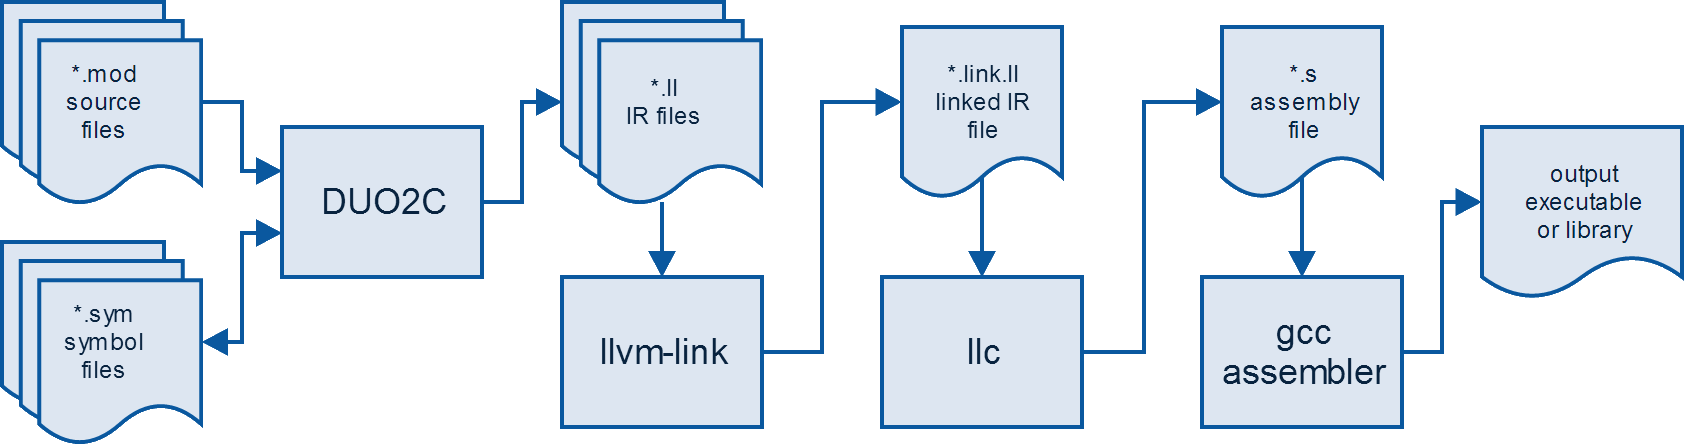
\includegraphics[width=\textwidth]{compiler}
    \caption{The compilation pipeline used by our compiler, where \emph{llvm-link} is the LLVM linker, and \emph{llc} is the LLVM compiler.}
    \end{figure}

    This document will outline the proposed additions to the language and provide examples of the new syntax's usage. For both of the extensions, care has been taken to follow the design principles employed by Oberon where possible. The rest of the language as implemented in the compiler adheres to the 1993 report on Oberon-2\cite{oberspec}.

    \section{External Interface Extension}
    To declare the existence of an external symbol to be linked, an \emph{EXTERNAL} keyword has been added. This keyword, followed by a string literal specifying the external symbol's identifier, may replace the body of a procedure. An optional \emph{IMPORT} keyword may also be used to import symbols from Dynamic Link Libraries on Windows, and translates to the \emph{dllimport} flag used by LLVM. When using the compiler, the libraries that contain definitions for external symbols can be specified in the same style as the GCC \emph{-l} option.

    \begin{figure}[!htbp]
    \begin{lstlisting}
        ExternalDecl = PROCEDURE IdentDef [FormalPars] ";"
                       EXTERNAL [IMPORT] string.
    \end{lstlisting}
    \caption{The formal syntax for an external declaration. The tokens \emph{IdentDef}, \emph{FormalPars}, and \emph{string} are as defined in the Oberon-2 specification\cite{oberspec}.}
    \end{figure}

    \noindent
    This declaration has the same header format as a normal procedure definition, but with the external reference in the place of a body. The following is an example of how this new syntax is used, to refer to a symbol from the OpenGL Utility Toolkit\cite{glut}. The command line arguments used to link with this library will contain \emph{-lglut} (or alternatively \emph{-l glut}, for POSIX compliance), just like with GCC.

    \begin{figure}[!htbp]
    \begin{lstlisting}
        PROCEDURE InitWindowSize* (width, height : INTEGER);
        EXTERNAL IMPORT "glutInitWindowSize";
    \end{lstlisting}
    \caption{An example of an externally defined procedure declaration.}
    \end{figure}

    \begin{figure}[!htbp]
    \begin{lstlisting}
        extern void __declspec(dllimport)
            glutInitWindowSize(int width, int height);
    \end{lstlisting}
    \caption{The original C declaration of the imported symbol\cite{gluth} when compiled on Windows.}
    \end{figure}

    \noindent
    Arguments of primitive types such as numerics and booleans are passed directly to the called procedure, but more complex types such as arrays and records are implicitly marshalled. The compiler stores an array as a pair of the array size and a pointer to the first element, which is marshalled by only sending the element pointer. Records contain a pointer to their corresponding virtual table used when dynamically dispatching bound procedure calls, and this will be stripped when marshalling records for use as arguments in external procedures.

    \section{SIMD Vector Extension}
    This second language extension adds some support for declaring and using vectors of primitive types, for systems that support Single Instruction Multiple Data (SIMD) operations. High level languages rarely support this technique, let alone feature it as a part of their syntax. Central to this extension is the addition of a new \emph{VECTOR} data type, which may substitute any primitive type.

    \begin{figure}[!htbp]
    \begin{lstlisting}
        VectorType    = VECTOR ConstExpr OF PrimitiveType.
        PrimitiveType = LONGINT  | INTEGER | SHORTINT
                      | LONGREAL | REAL 
                      | BOOLEAN  | SET     | CHAR.
    \end{lstlisting}
    \caption{The formal syntax for the \emph{VECTOR} type.}
    \end{figure}

    \noindent
    Additionally, a vector literal may be used which is a list of expressions surrounded by angle braces.
    
    \begin{figure}[!htbp]
    \begin{lstlisting}
        Vector   = "<" ExprList ">".
        ExprList = Expr {"," Expr}.
    \end{lstlisting}
    \caption{The formal syntax for a vector literal.}
    \end{figure}

    \noindent
    Any operators applied to vectors are implicitly applied to each element of the vector independently. For systems that support it, these operations are parallelised as SIMD instructions by LLVM. These expressions are checked at compile time to ensure the vector sizes match, and the element types are compatible. For operations applied to a vector and a literal, the literal is implicitly promoted to a vector with the same number of elements as the other operand, where each element is the literal's original value.

    \begin{figure}[!htbp]
    \begin{lstlisting}
        VAR a, b : VECTOR 4 OF INTEGER;
        BEGIN
            a := 4;             (* set every element of a to 4  *)
            b := <1, 2, 3, 4>;  (* assign a vector literal to b *)
            a := a + b * 2;     (* a is now <6, 8, 10, 12>      *)
        END;
    \end{lstlisting}
    \caption{An example of operations applied to vectors.}
    \end{figure}

    \noindent
    Individual elements of a vector may be accessed or assigned to with the same syntax as array indexing.

    \begin{figure}[!htbp]
    \begin{lstlisting}
        a[0] := 12;
        a[1] := a[0] * a[2];
        b    := <a[3], a[2], a[1], a[0]>;
    \end{lstlisting}
    \caption{An example of indexing elements of a vector.}
    \end{figure}

    \noindent
    Finally, two procedures to transfer elements of vectors to and from arrays are provided, \emph{VECLOAD} and \emph{VECSTORE}.

    \begin{figure}[!htbp]
    \begin{lstlisting}
        VECLOAD(a, c, 2);  (* fill vector a with values from
                            * array c starting at index 2    *)

        VECSTORE(b, c, 0); (* store elements from vector b in
                            * array c starting at the first index *)
    \end{lstlisting}
    \caption{Examples of \emph{VECLOAD} and \emph{VECSTORE}.}
    \end{figure}

    \begin{thebibliography}{9}
        \bibitem{llvmusers}
            \emph{LLVM Users}. \newline
            \url{http://llvm.org/Users.html}
            [Retrieved \today].

        \bibitem{oberspec}
            Hanspeter M\"{o}ssenb\"{o}ck, Niklaus Wirth,
            \emph{The Programming Language Oberon-2}. \newline
            \url{http://cseweb.ucsd.edu/~wgg/CSE131B/oberon2.htm}
            [Retrieved \today].

        \bibitem{glut}
            Khronos Group,
            \emph{GLUT - The OpenGL Utility Toolkit}. \newline
            \url{http://www.opengl.org/resources/libraries/glut/}
            [Retrieved \today].

        \bibitem{gluth}
            Khronos Group,
            \emph{glut.h} \newline
            \url{http://www.cs.uaf.edu/~cs381/GLUT/glut.h}
            [Retrieved \today].

    \end{thebibliography}
\end{document}
